\documentclass[11pt]{article}
\usepackage{graphicx}
\usepackage[portuguese]{babel}
\usepackage[colorlinks]{hyperref}
\usepackage[margin=1in]{geometry}

\title{\bf Movimento Browniano em 2D}
\author{Jo\~{a}o Bravo, 84390 \& Carolina Martins, 84374\\MEFT}
\date{Janeiro 2016}

\begin{document}
\maketitle
\begin{center}

\includegraphics[scale=0.08]{IST_Logo}
\end{center}
\noindent\hrulefill

\section*{$\quad$ Introdu\c{c}\~{a}o}
\begin{quote}
 \qquad Estudado pela primeira vez em 1827 por Robert Brown, o movimento browniano consiste no deslocamento aleat\'{o}rio de part\'{i}culas em suspens\~{a}o num meio fluido devido aos choques entres as mesmas.
 \par
 \qquad Com este programa, pretendemos simular o movimento browniano a duas dimens\~{o}es atrav\'{e}s de colis\~{o}es el\'{a}sticas entre um c\'{i}rculo, an\'{a}logo a uma part\'{i}cula, e um conjunto de c\'{i}rculos relativamente menores, an\'{a}logos \'{a}s part\'{i}culas constituintes do fluido circulante, com a possibilidade de manipular as suas principais carater\'{i}sticas: o raio, a massa e a sua velocidade inicial.
\end{quote}

\begin{figure}[hb]
\centering
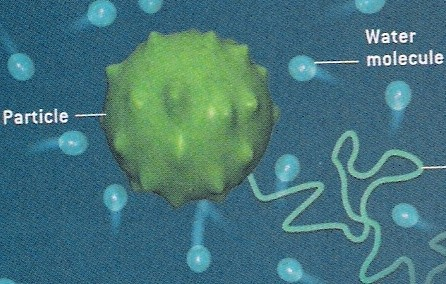
\includegraphics[scale=1]{brownian}
\caption{\footnotesize Movimento Browniano entre uma part\'{i}cula e mol\'{e}culas de \'{a}gua}
\end{figure}

\newpage

\section*{$\quad$ Funcionamento do Programa}
\begin{quote}
 Divindo o a estrutura do programa em sec\c{c}\~{o}es para facilitar a compreens\~{a}o do mesmo:
 \begin{itemize}
 \item Na sec\c{c}\~{a}o {\color{red} 1}, pode fechar o programa ou obter informa\c{c}\~{o}es \`{a} cerca da produ\c{c}\~{a}o do mesmo;
 \item Na sec\c{c}\~{a}o {\color{red} 2}, tem controlo total sobre os aspetos relativos \`{a}s coliso\~{e}s j\'{a} falados bem como o n\'{u}mero de part\'{i}culas do fluido simulado;
 \item Na sec\c{c}\~{a}o {\color{red} 3}, pode iniciar e pausar o movimento. Para reiniciar todos os valores basta carregar no bot\~{a}o \textit{RESET};
 \item Na sec\c{c}\~{a}o {\color{red} 4}, pode controlar o par de coordenadas (\textit{x, y}) relativas \`{a} posi\c{c}\~{a}o do c\'{i}rculo grande. Esta posi\c{c}\~{a}o tamb\'{e}m \'{e} reiniciada ao carregar no bot\~{a}o \textit{RESET};
 \item A sec\c{c}\~{a}o {\color{red} 5} permite-lhe visualizar a velocidade do c\'{i}rculo grande em tempo real ou esconder todos os c\'{i}rculos pequenos;
 \item Finalmente, na sec\c{c}\~{a}o {\color{red} 6}, tem a possibilidade de escolher diferentes cores para os c\'{i}rculos e fundo bem como v\'{a}rios temas personalizados para o programa. Novamente, estas carater\'{i}sticas podem ser reiniciadas pelo bot\~{a}o \textit{RESET}.
\end{itemize}
\end{quote}

\begin{figure}[hb]
\centering
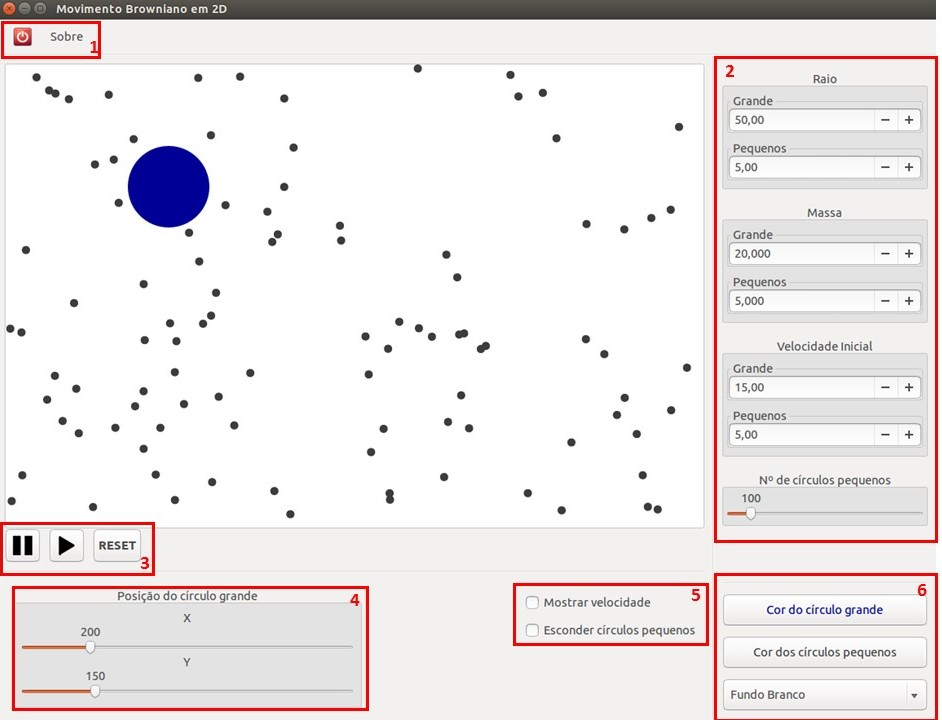
\includegraphics[scale=0.4]{tela}
\end{figure}

\begin{quote}
 \qquad De notar ainda que pode arrastar o c\'{i}rculo grande com o rato e alterar quaisquer valores em qualquer altura, mesmo com o movimento iniciado.
\end{quote}

\end{document}
